% this section describes the computational image complexity analysis
%!Concise version
The theory framework section meticulously examined the architectural evolution, revealing a recurring cycle oscillating between complex and simple styles.
Given the recent technological advancements and contemporary architectural trends, there is a compelling indication that the present era is poised for a shift toward complexity, countering the preceding Modernist movement characterized by minimalism and simplicity.

In pursuit of validating this hypothesis, we developed a Computational Image Complexity Analysis (CICA) system.
Our primary objective was to not only empirically validate the trends in architectural complexity suggested by our theoretical analysis but also to create a quantifiable metric.
This metric would play a crucial role in evaluating and ranking the 3D-modeled facades intended for use in the Virtual Reality experience.

The Computational Image Complexity  Analysis (CICA) system is a Python function that assesses complexity by quantifying the number of elements within a building's design and analyzing their shapes.
The higher the count of elements, the higher the assigned complexity score, and vice versa.
This approach draws inspiration from Venturi et al.'s reflection on complexity, as articulated in their work\cite{Venturi1977}.
They posited that a building's complexity could be gauged by the time it takes to mentally process and form a coherent image of its constituent elements.
This fundamental concept underpins the CICA system's methodology(Figure\ref{fig:ImageComplexityAnalysisFlowchart}).


The CICA system evaluates complexity through two metrics: edge density, using the Canny Edge Detection algorithm\cite{EdgeOpenCV2023}, and contour count, based on contour approximation\cite{ContourOpenCV2023}.
These metrics are normalized and combined into a unified complexity score (Table\ref{tab:MetricsandWeights}).

The complexity scoring function \(f_1(x)\) is a crucial part of our CICA system, where the weighted sum of the normalized scores for each metric is calculated, providing an overall complexity score for each building image (Table\ref{tab:ComplexityScoreFunction_table}).

In summary, the CICA system leverages two key metrics, edge density and contour count, to quantify the complexity of building facades.
While edge density emphasizes the presence and density of edges, contour count delves into the intricacies of the shapes represented by these edges.
The combination of these metrics provides a more comprehensive and nuanced assessment of architectural complexity, making them valuable tools in our analysis.
Having outlined the development and purpose of the Computational Image Complexity Analysis (CICA) system, we will now delve into its application.

The CICA system's first application is the historical analysis of 180 buildings from various architectural eras (Figure \ref{fig:CICAHistoryPlot}), resulting in a scatter graph demonstrating complexity trends over time.

The second application involves ranking 3D-modeled facades for the VR experiment.
Using Blender, we modeled facades with varying complexity, categorized into ten levels based on CICA scores (Figure\ref{fig:CICARenderPlot}).
Through CICA, we aim to empirically validate architectural complexity trends and effectively prepare for the VR experiment that assesses user perceptions of facade complexity.
This dual application of the CICA system allows us to quantitatively explore architectural complexity, aligning with our theoretical analysis and providing a basis for further experimentation in VR


%!Original text
%The theory framework section meticulously examined the architectural evolution, revealing a recurring cycle oscillating between complex and simple styles.
%Given the recent technological advancements and contemporary architectural trends, there is a compelling indication that the present era is poised for a shift toward complexity, countering the preceding Modernist movement characterized by minimalism and simplicity.
%
%In pursuit of validating this hypothesis, we developed a Computational Image Complexity Analysis (CICA) system.
%Our primary objective was to not only empirically validate the trends in architectural complexity suggested by our theoretical analysis but also to create a quantifiable metric.
%This metric would play a crucial role in evaluating and ranking the 3D-modeled facades intended for use in the Virtual Reality experience.
%
%The Computational Image Complexity  Analysis (CICA) system is a Python function that assesses complexity by quantifying the number of elements within a building's design and analyzing their shapes.
%The higher the count of elements, the higher the assigned complexity score, and vice versa.
%This approach draws inspiration from Venturi et al.'s reflection on complexity, as articulated in their work\cite{Venturi1977}.
%They posited that a building's complexity could be gauged by the time it takes to mentally process and form a coherent image of its constituent elements.
%This fundamental concept underpins the CICA system's methodology(Figure\ref{fig:ImageComplexityAnalysisFlowchart}).
%
%%% Figure Computational Image Compexity Analysis (CICA) System flowchart
%    \begin{figure}[!htb]
%      \centering
%      % trim=left 190 down 250 right 150 top5
%      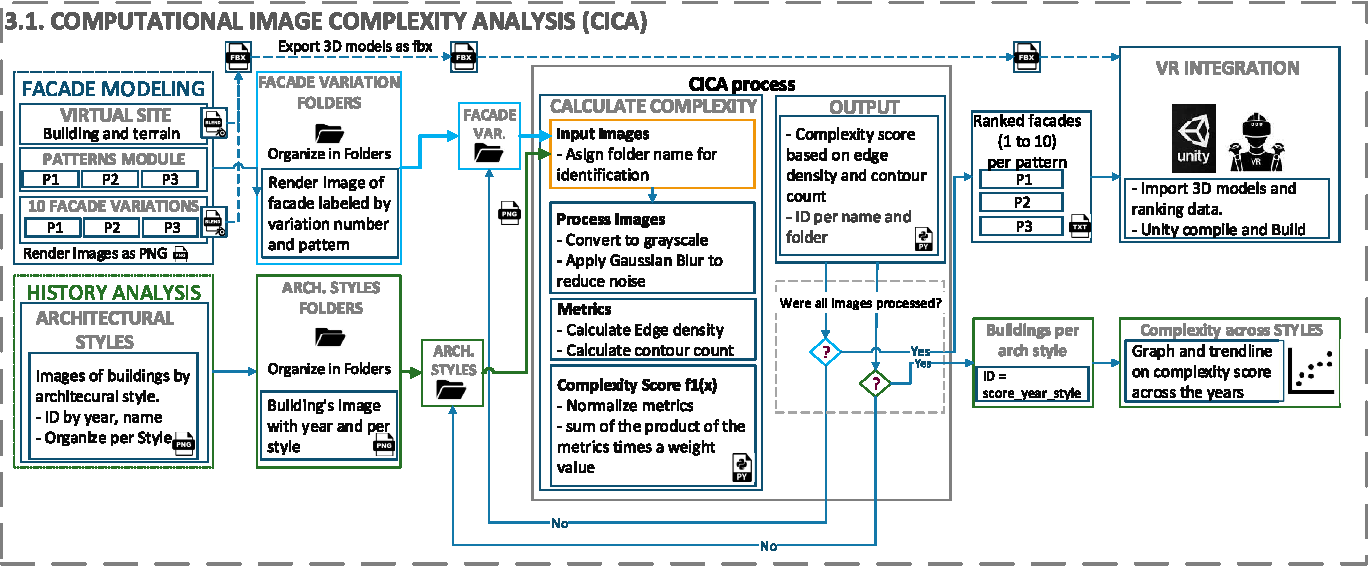
\includegraphics[width= \linewidth, trim=0 0 0 0, clip]{Images/ImageComplexityAnalysisFlowchart}
%      \caption{Flowchart illustrating the applications of Computational Image Complexity Analysis, including its role in analyzing complexity scores for historical architectural styles and ranking modeled facades for the VR Building Complexity System.}
%      \label{fig:ImageComplexityAnalysisFlowchart}
%    \end{figure}
%
%The Computational Image Complexity Analysis (CICA) system as shown in Figure\ref{fig:ImageComplexityAnalysisFlowchart} works by using building images as input, subsequently processing these images to enhance contrast and minimize noise, thereby improving the recognition of individual elements within the building's design.
%
%The system employs a method of complexity quantification based on two metrics: edge density and contour count .
%They were chosen by their capabilities in computer vision for identifying edges and shape analysis and whose results are later combined into a unified `complexity score'(see \ref{tab:MetricsandWeights}).
%
%    %%Table: Performance Indicators
%    \begin{table*}[htb]
%        \centering
%        \small
%        \caption{Metrics and weights for the calculation of the `Complexity score'}
%        \label{tab:MetricsandWeights}
%        \begin{tabularx}{\textwidth}{p{3.5cm} p{1cm} X X p{1cm}}
%            \toprule
%            \textit{Complexity metric} &
%              \textit{N} &
%              \textit{Metric name/description} &
%              \textit{Quantitative   method} &
%              \textit{Weights} \\ \midrule
%            \textbf{Edge Density} &
%              1 &
%              Edge detection using Canny Edge Detection algorithm for highlighting the most relevant features of a building.
%                &
%              Measured by dividing the number of non-zero (edge) pixels in the edges image by the total number of pixels in the image.
%                &
%              8\\
%            \textbf{Contour count} &
%              2 &
%              Employs contour approximation algorithm for shape analysis to determine intricacy of edges.
%                &
%              Measure by counting the number of segments in an edge.
%                &
%              2\\ \bottomrule
%               &
%               &
%              \textbf{TOTAL} &
%              &
%              \textbf{10}\\ \bottomrule
%        \end{tabularx}
%    \end{table*}
%
%In the case of edge density, the system utilizes edge detection, to highlight a pronounced edge within an image of a building.
%This can be associated with a distinct element of the building, and in the case of more intricate structures, this script interprets such edges as separations denoting additional architectural elements.
%
%Edge detection is a critical step in our Computational Image Complexity Analysis (CICA) system, performed using the Canny Edge Detection algorithm\cite{EdgeOpenCV2023}.
%This algorithm, readily accessible in Python through OpenCV (cv2.Canny function), is designed for computer vision tasks and excels at identifying edges within an image.
%It achieves this by identifying regions of the image where there is a rapid change in intensity, often corresponding to object boundaries or significant features.
%The outcome of this process is an abstraction that highlights the most relevant features of the building, in a binary image (black and white) as demonstrated in the third panel in Figure\ref{fig:ComplexityPlotHistory}.
%
%%%Figure Canny Edge of historic buildings
%     \begin{figure}[htb]
%          \centering
%          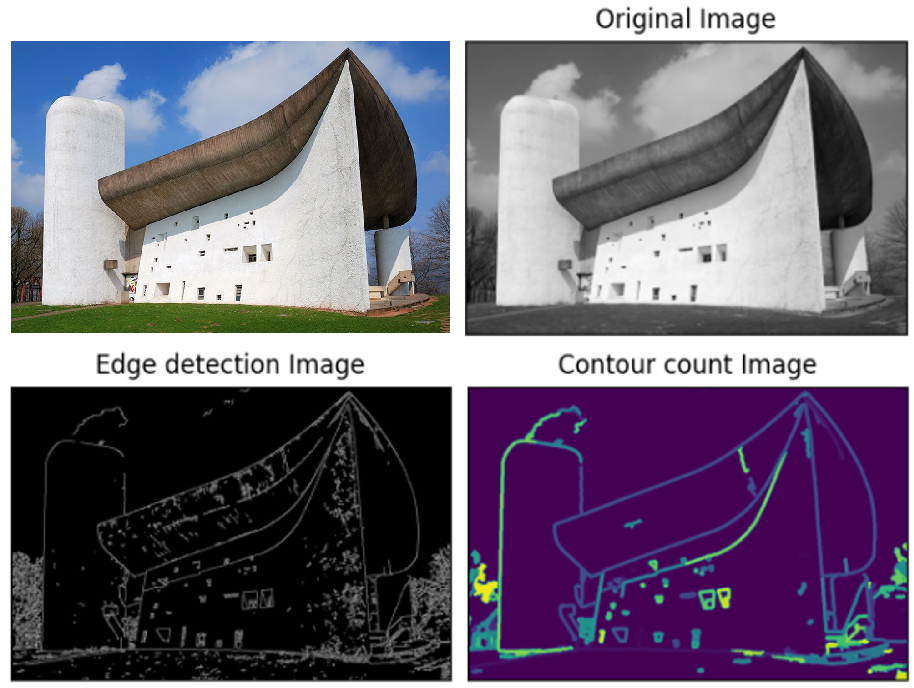
\includegraphics[width= \linewidth]{Images/ComplexityPlotHistoryCICA}
%          \caption{Comparison of images of Chapelle Notre-Dame-du-Haut de Ronchamp, constructed in 1955. Clockwise from the upper-left: the original image, its corresponding denoised Grayscale version, the binary image used for edge density analysis, and the contour count image. The Edge Detection Plot highlights architectural features, while contour count aids in shape analysis within the building's design.}
%          \label{fig:ComplexityPlotHistory}
%        \end{figure}
%
%The edge density is subsequently computed by dividing the number of non-zero (edge) pixels in the edges image by the total number of pixels in the original image.
%This calculation provides a measure of how much of the image consists of edges, resulting in an edge density score that serves as a proxy for complexity.
%
%The second metric, known as contour count, plays a crucial role in computing the complexity score of a building within our CICA system.
%This metric was incorporated to address a potential limitation of edge density: the possibility of misjudging complexity when intricate and simple curves share similar edge densities, potentially leading to erroneous complexity assessments.
%
%The contour count metric employs the contour approximation algorithm, a valuable tool for shape analysis and object recognition\cite{ContourOpenCV2023}.
%Implemented through Python's OpenCV library (specifically, the cv2.findContours() function), this algorithm operates on binary images (black and white), which are obtained by processing the original image through the Canny Edge Detection algorithm (see the third panel in Figure \ref{fig:ComplexityPlotHistory}).
%
%Unlike edge density, which quantifies the presence of edges and their density, the contour count metric focuses on delineating the boundaries of shapes within the image.
%It achieves this by identifying straight lines and approximating contours, eliminating redundant points and retaining only the endpoints\cite{ContourOpenCV2023}.
%This approach allows us to efficiently count the number of segments present in an edge, providing a more nuanced assessment of complexity.
%
%The contour count metric is computed by counting the number of contours present in the image.
%This calculation offers insights into the intricacy of the shapes represented by the most relevant edges within a building's design, as illustrated in the fourth panel in Figure\ref{fig:ComplexityPlotHistory}.
%
%Both the `Edge density metric' and the `Contour Count metric' metrics are normalized within the range [0, 1], a process that involves extracting the minimum and maximum values from all the images in the dataset for both operations.
%These normalized scores are then subjected to a `Complexity Scoring' function \(f_1(x)\) (as detailed in Table \ref{tab:ComplexityScoreFunction_table}).
%
%    %f1: Complexity scoring function
%    \begin{table}[htb]
%        \caption{Complexity scoring function }
%        \label{tab:ComplexityScoreFunction_table}
%        \centering
%        \small
%        \begin{tabular}{|p{8cm}|}
%        \hline
%            \textbf{\(f_1\), Unified `Complexity Scoring' function 1}\\
%            \textit{Calculate the complexity score for all the images on the data pool}
%            \\
%            \begin{equation}
%                f_1(x) = \left[ \mathrm{round}\left(\sum_{i=1}^{n} w_i \cdot a_i, 2\right) \right] = complexity\_score
%            \label{eq:F1_ComplexityScoreFunction}
%            \end{equation}
%
%            \\
%            \textit{ for the Buildings included in the database.}\\
%            \\
%            \textit{where;} \\
%            \\
%            \(n \); is the number of performance indicators \\
%            \(w_i \); represents the i-th elements weight input and \\
%            \(a_i \); represents the i-th normalized score for the respective metric(`Edge Density' and `Contour Count').\\
%            \\
%
%            \textit{Finally, the `Complexity score' is assigned to each building for data visualization.}\\
%        \hline
%        \end{tabular}
%    \end{table}
%
%Table \ref{tab:ComplexityScoreFunction_table} outlines the complexity scoring function \(f_1(x)\), which calculates the complexity score for all the images in the dataset.
%It involves taking the weighted sum of the normalized scores for each metric (edge density and contour count) and rounding the result to two decimal places.
%This `complexity score' is subsequently assigned to each building image for data visualization.
%
%
%This function\ref{eq:F1_ComplexityScoreFunction} takes into account the individual scores obtained for each metric and multiplies them by the pre-determined weights assigned to each metric.
%The weighted scores are then summed together to calculate a `complexity score' for each building image.
%
%In summary, the CICA system leverages two key metrics, edge density and contour count, to quantify the complexity of building facades.
%While edge density emphasizes the presence and density of edges, contour count delves into the intricacies of the shapes represented by these edges.
%The combination of these metrics provides a more comprehensive and nuanced assessment of architectural complexity, making them valuable tools in our analysis.
%
%Having outlined the development and purpose of the Computational Image Complexity Analysis (CICA) system, we will now delve into its application.
%
%%! section on CICA applied to historical analysis
%First, we will employ the CICA system to quantify the complexity score for a selection of renowned buildings representing different architectural eras and styles (Figure \ref{fig:ComplexityPlotHistory}).
%
%This comprehensive dataset includes a total of 180 buildings, meticulously organized according to architectural style, with an average of 10 buildings per style, each labeled with its name and year of construction (as illustrated in Figure \ref{fig:ImageComplexityAnalysisFlowchart}).
%
%This analytical endeavor will culminate in the creation of a scatter graph, thoughtfully color-coded to distinguish architectural styles, and accompanied by a trendline.
%Together, these visualizations aim to provide a clear depiction of the trends in complexity across the years.
%
%By categorizing data per architectural style and era, we intend to substantiate whether a cyclical pattern indeed exists in architectural design throughout history.
%Furthermore, this analysis will offer empirical evidence regarding the contemporary architectural shift towards more intricate and complex designs, aligning with the conclusions drawn from our theoretical examination.
%
%%!Section on CICA applied for 3d modeled facades ranking
%
%With the first application of the Computational Image Complexity Analysis (CICA) system shedding light on the historical trends in architectural complexity, we now pivot our focus to the second application of this tool.
%In this phase, the CICA system will be harnessed for a distinct purpose: the ranking of 3D-modeled facades (Figure\ref{fig:ComplexityPlotRenderCICA}).
%
%As part of our upcoming Virtual Reality (VR) experiment, participants will interact with facades showcasing varying levels of complexity.
%These facades will play a pivotal role in our upcoming Virtual Reality (VR) experiment, where participants will engage with facades featuring varying levels of complexity.
%
%To facilitate this experiment effectively, we have adapted the CICA system to assess the complexity of facade variations representing three distinct patterns, all modeled in Blender.
%These variations are then categorized into 10 distinct levels of complexity, determined by the complexity scores generated by the CICA system.
%
%%%Figure Canny Edge of render buildings
%     \begin{figure}[htb]
%          \centering
%          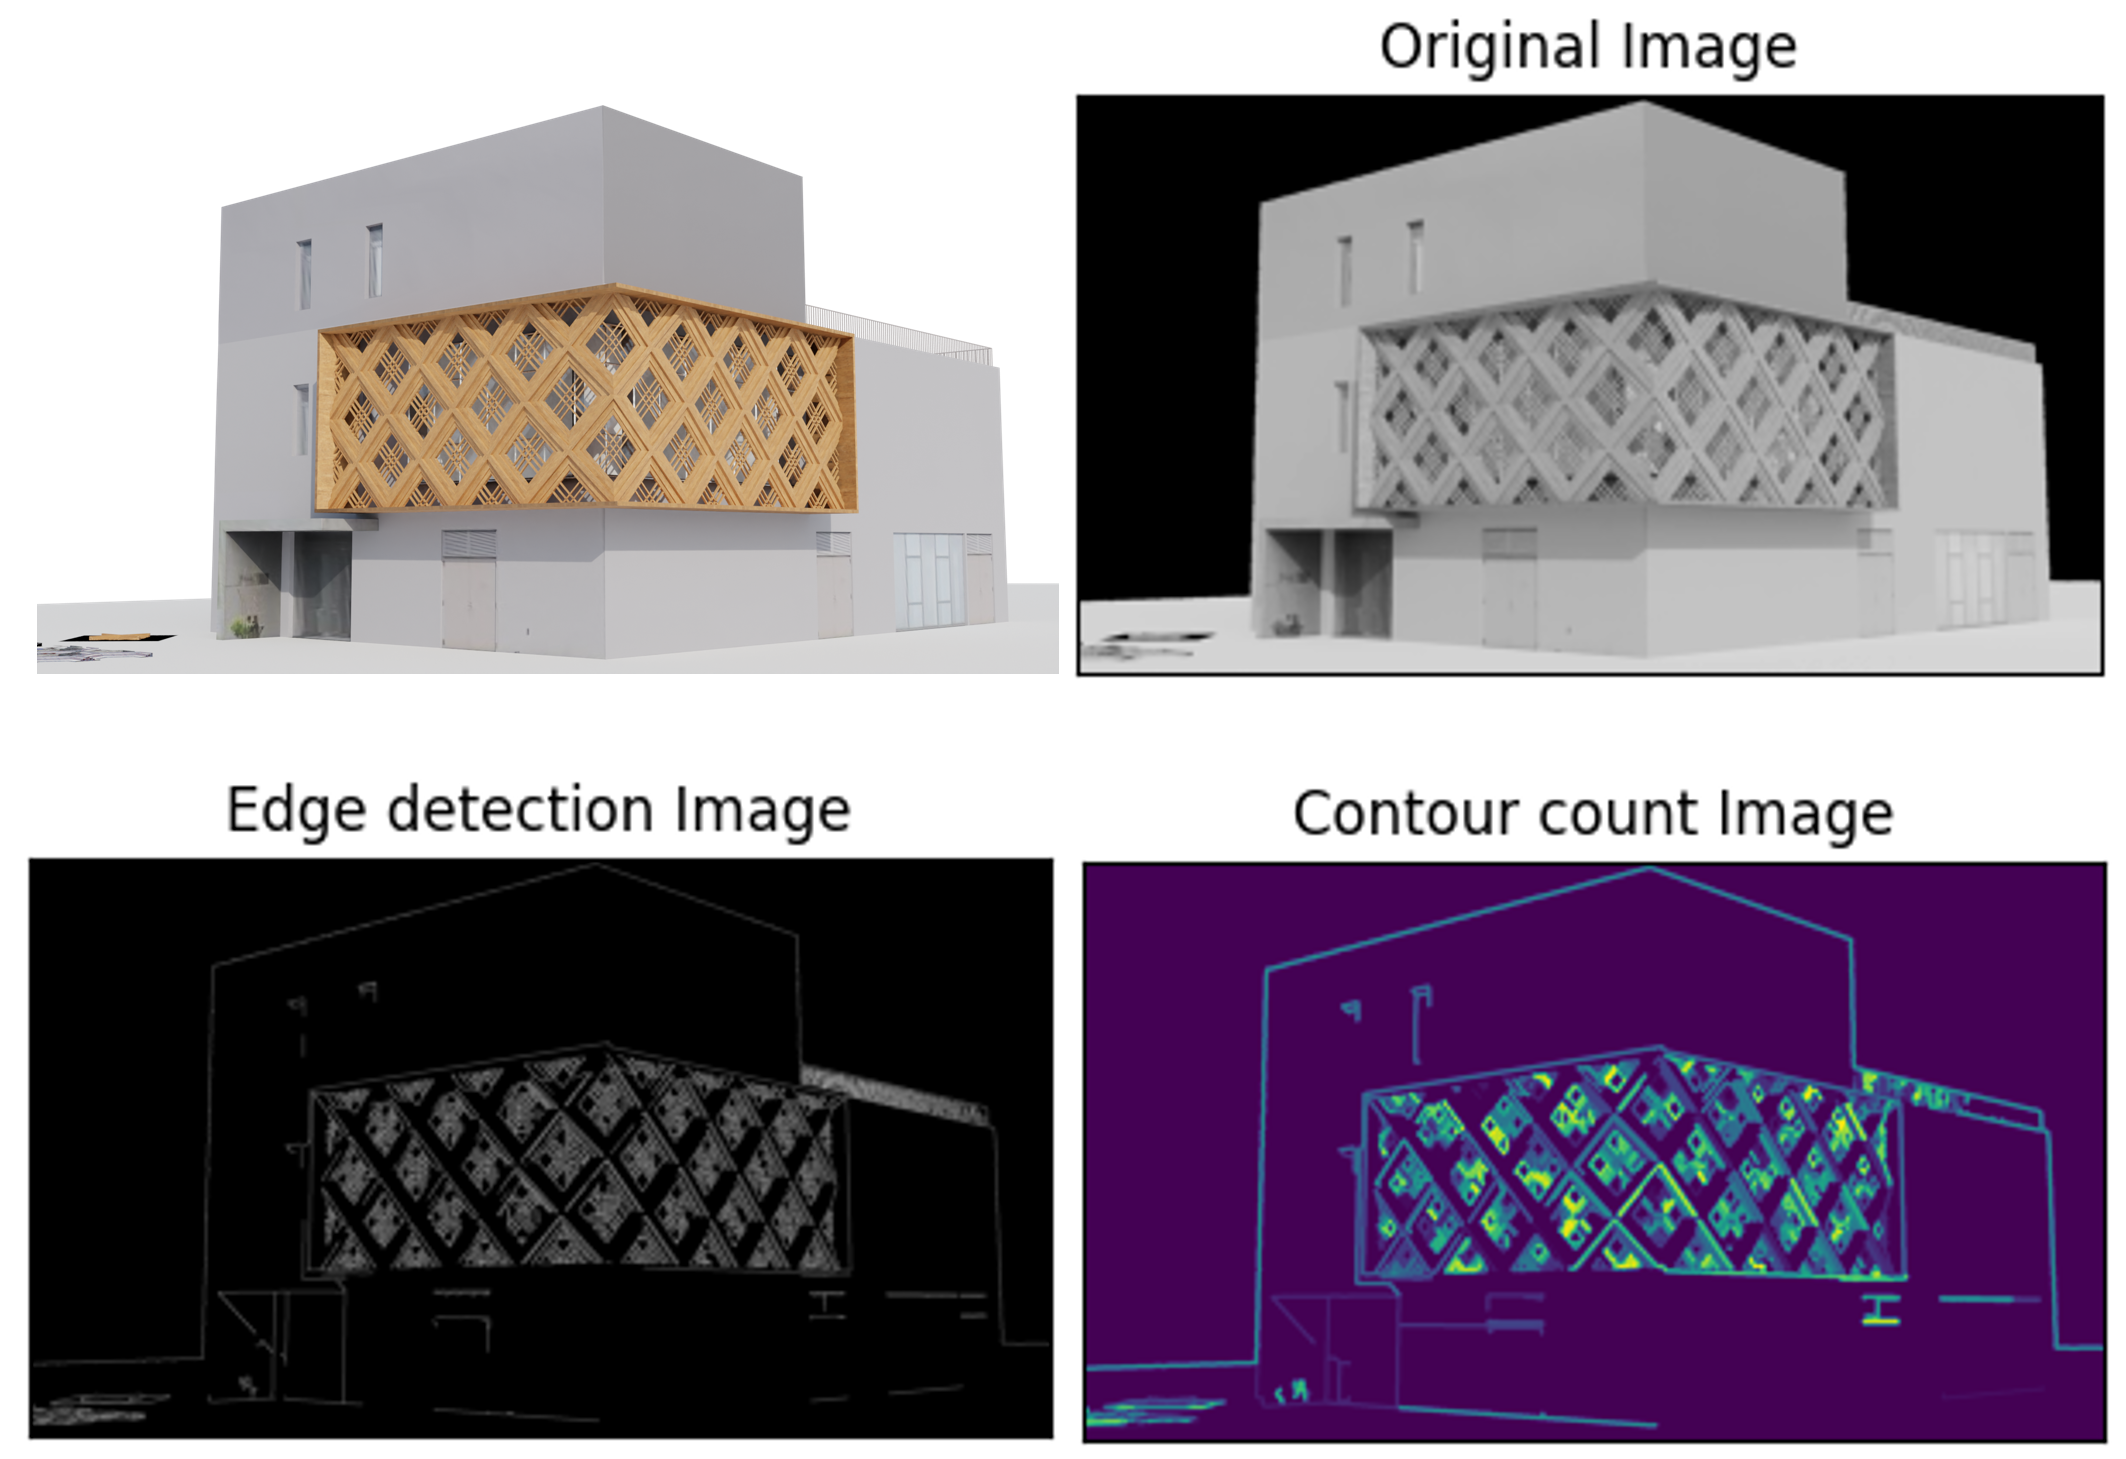
\includegraphics[width= \linewidth]{Images/ComplexitPlotRenderCICA}
%          \caption{Comparison of images of render of facades variation modeled in blender for the VR complexity analysis system used on this research. Clockwise from the upper-left: the original image, its corresponding denoised Grayscale version, the binary image used for edge density analysis, and the contour count image. The Edge Detection Plot highlights architectural features, while contour count aids in shape analysis within the building's design.
%          }
%          \label{fig:ComplexityPlotRenderCICA}
%        \end{figure}
